%# -*- coding:utf-8 -*-
\documentclass[10pt,aspectratio=169,mathserif]{beamer}		
%设置为 Beamer 文档类型,设置字体为 10pt,长宽比为16:9,数学字体为 serif 风格

%%%%-----导入宏包-----%%%%
\usepackage{zju}			%导入 zju 模板宏包
\usepackage{ctex}			%导入 ctex 宏包,添加中文支持
\usepackage{amsmath,amsfonts,amssymb,bm}   %导入数学公式所需宏包
\usepackage{color}			 %字体颜色支持
\usepackage{graphicx,hyperref,url}
\usepackage{metalogo}	% 非必须
\usepackage{ragged2e}
%% 上文引用的包可按实际情况自行增删
%%%%%%%%%%%%%%%%%%
\usepackage{fontspec}
\usepackage{xeCJK}
% \setCJKmainfont{Source Han Sans SC}
\usepackage{pgfplots}
\pgfplotsset{compat=1.18}


\beamertemplateballitem		%设置 Beamer 主题

%%%%------------------------%%%%%
\catcode`\。=\active         %或者=13
\newcommand{。}{.}				
%将正文中的“。”号转换为“.”。中文标点国家规范建议科技文献中的句号用圆点替代
%%%%%%%%%%%%%%%%%%%%%

%%%%----首页信息设置----%%%%
\title[12-11]{遗传算法欺骗问题}
\subtitle{及其优化策略}			
%%%%----标题设置


\author[罗俊勋]{
  {\small \url{junxun-luo@outlook.com}}}
%%%%----个人信息设置
  
\institute[IOPP]{
  School of mathmatics\\ 
  Zhejiang University}
%%%%----机构信息

\date[2024-12-11]{
  2024年12月11日}
%%%%----日期信息
  
\begin{document}

\begin{frame}
	\titlepage
\end{frame}				%生成标题页


\begin{frame}
%%  	\frametitle{提纲}
	\tableofcontents
\end{frame}				%生成提纲页

\section{介绍}
\begin{frame}
	\frametitle{遗传算法欺骗问题}
	将所有妨碍适应度高的个体的生成从而影响算法正常工作的问题统称为遗传算法的欺骗问题
	\begin{itemize}
		\item 性质不好的函数(例如不连续,多峰值,有跳跃点)

		\item 编码设计问题
		
		\item ...
	\end{itemize}
	
下面都以求解这个函数的最大值为例来说明如何提升遗传算法的求解性能
\[ f(x,y) = 
\begin{cases}
	   \sin(\frac{\pi}{3}x)\sin(\frac{\pi}{3}y) + \cos(\frac{\pi}{4}x)\cos(\frac{\pi}{4}y) + 4 & |x|,|y| \leq \epsilon \\ 
	   \sin(\frac{\pi}{3}x)\sin(\frac{\pi}{3}y) + \cos(\frac{\pi}{4}x)\cos(\frac{\pi}{4}y) + 2 & \epsilon < |x|,|y| \leq 10 \\
\end{cases}
\]	

其中 $\sin(\frac{\pi}{3}x)\sin(\frac{\pi}{3}y) + \cos(\frac{\pi}{4}x)\cos(\frac{\pi}{4}y)$ 

在 $( 4.3222, 4.3222 )$ 处取到最值 $1.91$

$f$ 在 $x=y=\epsilon$ 时取到最值

\end{frame}

\section{欺骗问题改进策略}
\begin{frame}
	\frametitle{种群大小改进}
    {\small 采用浮点数编码、单点交叉、单点变异求解上述函数的最大值(取 $\epsilon = 0.1$)。 考察种群大小对求解效果的影响:}
\(ratio = \frac{\text{算法搜索到}\delta(0,\epsilon)^2\text{的次数}}{\text{算法执行次数}}\)

	\begin{figure}
		\centering
		\begin{minipage}{0.45\textwidth}
			\centering
			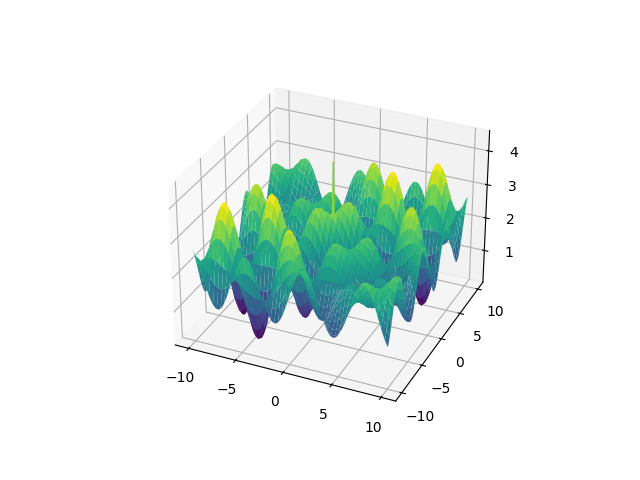
\includegraphics[width=\textwidth]{./img/Figure_1.png}
			% \caption{函数示意}
			\label{fig:figure1}
		\end{minipage}
		\hfill
		\begin{minipage}{0.50\textwidth}
			\centering
			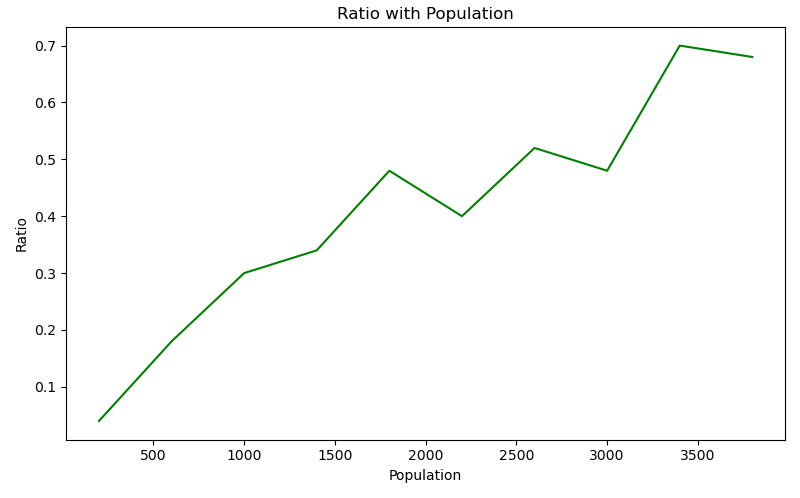
\includegraphics[width=\textwidth]{./img/Figure_3.png}
			% \caption{种群数量-找到最优解的比率}
			\label{fig:figure3}
		\end{minipage}
		\label{fig:figure_combined}

		可以看出, 随着种群大小的增加, 算法的搜索空间变得更大, 更容易搜索到全局最优解

	\end{figure}

\end{frame}


\begin{frame}
	\frametitle{编码方式改进举例}

	\begin{minipage}{0.45\textwidth} 
		比较二进制编码和浮点数编码的效果。

		在设定交叉概率 $p_c = 1$,变异概率 $p_m = 0.05$,种群数量 $600$,迭代次数 $200$ 的情况下
		
		分别运行 $1000$ 次程序比较二者求出最优解的比率:

		\begin{itemize}
			\item 浮点数编码: \textbf{ratio: 0.641}
			\item 二进制编码: \textbf{ratio: 0.076}
		\end{itemize}
	\end{minipage}
	\hfill
	\begin{minipage}{0.45\textwidth} % 右边图表占 45% 宽度
		\begin{tikzpicture}
		    \begin{axis}[
		        ybar,
		        symbolic x coords={浮点数, 二进制},
		        xtick=data,
		        bar width=12pt,
		        ymin=0, ymax=1,
		        nodes near coords,
		        nodes near coords align={vertical},
		        xlabel={编码方式},
		        ylabel={ratio},
		        enlarge x limits=0.3,
		        width=6cm,
		        height=4.5cm
		    ]
		        \addplot[
		            fill=blue!50
		        ] coordinates {
		            (浮点数, 0.641)
		            (二进制, 0.076)
		        };
		    \end{axis}
		\end{tikzpicture}
	\end{minipage}

\end{frame}

\begin{frame}
	\frametitle{变异策略改进}
	对单点变异、均匀变异和高斯变异进行比较。

	\begin{minipage}{0.60\textwidth} 
		\begin{figure}[h]
			\centering
			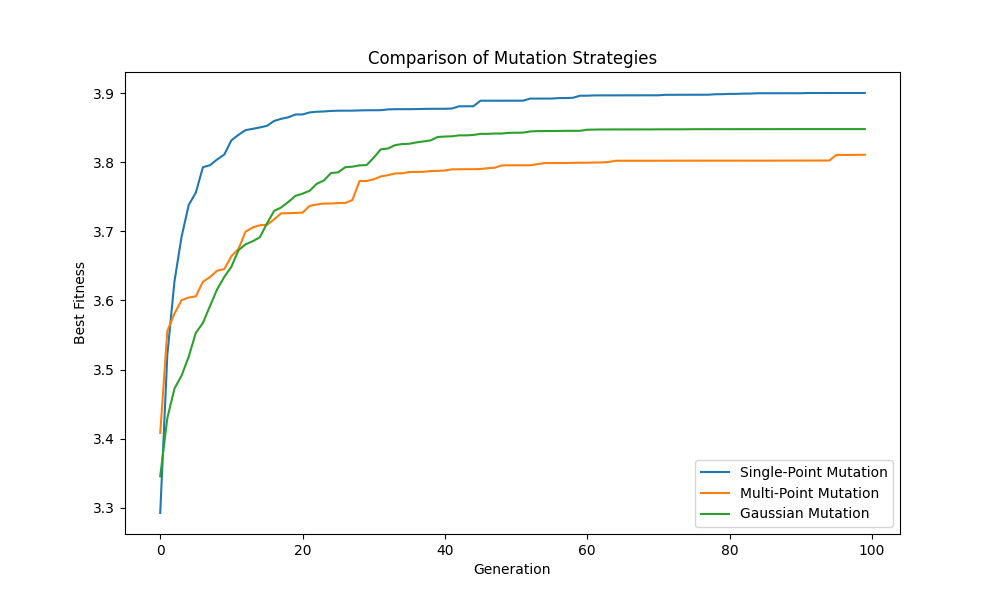
\includegraphics[width=0.9\textwidth]{img/Figure_4.png}
			\caption{不同变异策略的性能对比}
			\label{fig:report-2024-12-11}
		\end{figure}
	\end{minipage}
	\hfill
	\begin{minipage}{0.35\textwidth}
		\begin{itemize}
			\item $0.1_{(10)} = 0.00011001100..._{(2)}$
			\item 实际上,对求解有利的模式为:
			\begin{itemize}
				\item $0.00010*...$
				\item $0.0000*...$
				\item $0.00011000*...$
			\end{itemize}
			\item 在关键部分进行变异是最重要的。
		\end{itemize}
	\end{minipage}
\end{frame}

\begin{frame}
	\frametitle{动态变异策略}
	设定种群大小为 $20$,迭代次数 $200$,交叉概率 $p_c=0.8$,固定变异概率 ${p_m}_{fixed} = 0.05$,动态变异概率 ${p_m}_{dynamic} = 0.5 \cdot (1 - t/T)$。
	\begin{figure}[h]
		\centering
		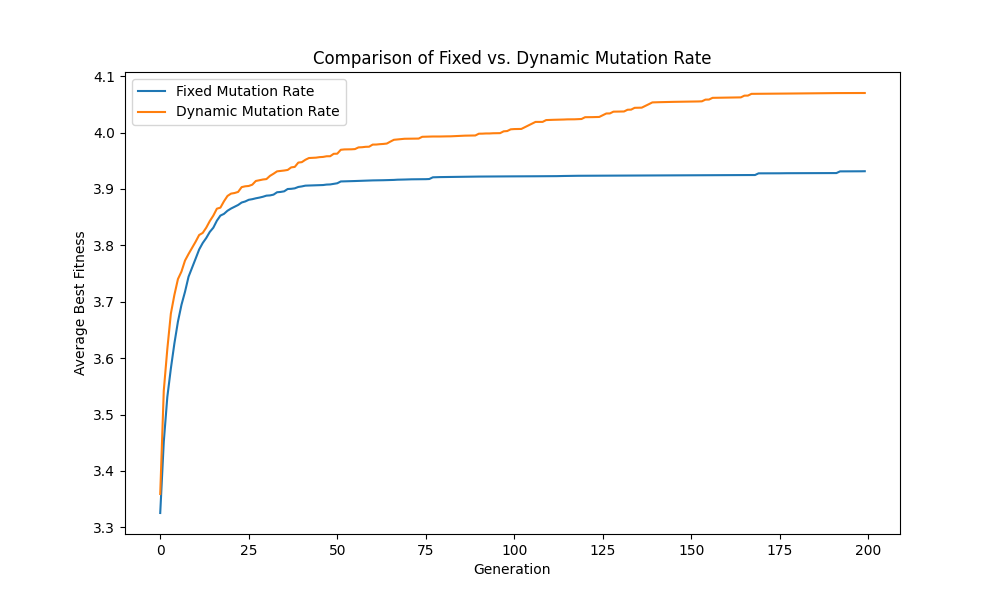
\includegraphics[width=0.6\textwidth]{img/Figure_5.png}
		\caption{动态变异策略的性能}
	\end{figure}	
\end{frame}

\section{总结}
\begin{frame}
	\frametitle{总结}
	\begin{itemize}
		\item 种群大小对搜索广度影响显著,尤其体现在算法运行初期(后期趋同)。
		\item 采用浮点数编码能显著提高算法性能,因其有助于群体稳定性。
		\item 变异策略需根据编码方式及问题特性进行调整。
		\item 动态变异策略能有效提升模型搜索能力。
	\end{itemize}
	
\end{frame}
	

\end{document}